\documentclass[conference]{IEEEtran}
\usepackage{cite}
\usepackage{amsmath,amssymb,amsfonts}
\usepackage{algorithmic}
\usepackage{graphicx}
\usepackage{textcomp}
\usepackage{xcolor}
\usepackage{fancyhdr}
\usepackage[hyphens]{url}

\def\BibTeX{{\rm B\kern-.05em{\sc i\kern-.025em b}\kern-.08em
    T\kern-.1667em\lower.7ex\hbox{E}\kern-.125emX}}

% Ensure letter paper
\pdfpagewidth=8.5in
\pdfpageheight=11in


%%%%%%%%%%%---SETME-----%%%%%%%%%%%%%
\newcommand{\iscasubmissionnumber}{NaN}
%%%%%%%%%%%%%%%%%%%%%%%%%%%%%%%%%%%%

\fancypagestyle{firstpage}{
}  


\pagenumbering{arabic}

%%%%%%%%%%%---SETME-----%%%%%%%%%%%%%
\title{CSE 240A Project Report: Branch Prediction} 
\author{Ke Wan, Xi Cai \\
Department of Computer Science \& Engineering \\
University of California San Diego

}
%%%%%%%%%%%%%%%%%%%%%%%%%%%%%%%%%%%%

\begin{document}
\maketitle
\thispagestyle{firstpage}
\pagestyle{plain}



%%%%%% -- PAPER CONTENT STARTS-- %%%%%%%%

\begin{abstract}

This document is intended to serve as a sample for submissions to the
47th IEEE/ACM International Symposium on Computer Architecture (ISCA),
May 30 -- June 3, 2020 in Valencia, Spain. This document provides
guidelines that authors should follow when submitting papers to the
conference.  This format is derived from the IEEE conference template IEEEtran.cls
file with the objective of keeping the submission similar to the final
version, i.e., the IEEEtran.cls template will also be used for
  the camera-ready version.

\end{abstract}

\section{introduction}
Branch predictor plays an important role on instruction sets. About 20\% of all computer instructions are branch instructions. However, branch instructions are
different from other kinds of instructions. There are multiple outcomes for a branch instruction. For example, for an \textbf{if-else} branch, there are two outcomes for this branch. 
If the value of the condition statement is true, then the program will execute the statements in the \textbf{if} code block. If not, the program will execute the statements
in the \textbf{else} code block. Predicting the outcome of branches correctly is important to accelerate the speed of instruction execution and reduce the overhead time. Therefore, branch
prediction strategy plays an important role in this task. 

In this paper, we introduce three branch predictors, G-Share branch predictor, Tournament branch
predictor, and custom Perceptron branch predictor. We discuss the structure, the design ideas, the implementation details of these three branch predictor.

G-Share predictor is the most simple branch predictor in this paper. It fetched the lowest 13-bit Program Counter(PC) and Global History Address(GHA). Then we did an XOR calculation for these two variables
and map the result to Prediction History Table(PHT) to fetch the 2-bit prediction result. 

Tournament branch predictor is a hybrid predictor. It contains a local branch
predictor, a global branch predictor, and a choice predictor. Firstly, the Tournament branch predictor will fetch the lowest 10 bits of global history as the index of choice prediction. Then the branch predictor 
will determine which branch predictor should be used. If the branch predictor chooses to use the local predictor, then it will firstly fetch the lowest 9-bit PC as the index of Local History Table(LHT), then it 
will fetch the 10-bit Local History(LH) from LHT as the index of 2-bit local prediction result. If the branch predictor chooses the global predictor, then
it will firstly get the lowest 10 bits global address as the index of global prediction table. Then it will fetch the 2-bit prediction result from global PHT.

Our custom Perceptron branch predictor is based on Perceptron Predictor~\cite{nicepaper4}, which contains 16 Preceptions to determine the prediction result. It contains a Table of Preceptron to store the perceptron weights for different local
history records and a register to store global history record. When the predictor encounters a branch, it will get the lowest 9 bits of PC address as the index of Perceptron Table. Then it will fetch the weights from the table and do
the prediction calculation using the formula $y_{out}=w_0+\sum_{i=1}^{n}{x_iw_i}$. If the value of $y_{out}$ is equal or greater than zero, then the branch predictor will predict it as TAKEN. Otherwise, the branch predictor will predict it as NOT-TAKEN. 

This paper also did experiments to test the prediction accuracy of three branch predictors on six address traces provided by instructors and made comparisons quantitatively. 
G-Share branch predictor achieves average accuracy of \textbf{94.41\%}. Tournament branch predictor achieves the average accuracy of \textbf{94.92\%}, a little better than G-Share predictor. 
The custom Perceptron branch predictor preforms the best among these three branch predictor. It has the average accuracy of \textbf{95.29\%}, and it beats the other two branch predictor in all six traces. 


\section{responsibility of each member}
This project is finished by two members, Ke Wan and Xi Cai. Ke Wan mainly contributes to design, develop, and test Tournament 
and custom Perceptron branch predictor. Xi Cai mainly contributes to develop G-share branch predictor and verified the 
correctness of our implementations. We cooperated to write project report. 

\section{background and motivation}
Branch predictor plays an important role on instruction sets. About 20\% of all computer instructions are branch instructions. However, branch instructions are
different from other kinds of instructions. There are multiple outcomes for a branch instruction. Predicting the outcome of branches correctly is important to accelerate the speed of instruction execution and reduce the overhead time. 
If we have an excellent branch predictor, then we will fetch the next instructions correctly in most of the time with less stall time. However, if we have a terrible branch predictor, then
we will find that the program will fetch wrong instructions in most of the time, which increases the execution time of the program. Therefore, having an excellent branch predictor can help us
accelerate the speed of the program further. This is our motivation to develop branch predictor. 

During lectures, Prof. Zhao showed us two simple but efficient branch predictors. One is G-Share branch predictor, and 
the other is Tournament branch predictor. We implemented both of them in this paper. However, Prof. Zhao encourages us to go further in this path. Therefore, we made research and decided to implement custom 
Perceptron branch predictor with a better performance. 

\section{design ideas}
The main task of a branch predictor is to predict whether or not the branch will be taken given the Program Counter(PC). Usually, a branch predictor maintains a global/local history table and a prediction table
in order to help predict the outcome of a branch. In this paper, we provide three branch predictors. They are G-Share branch predictor, Tournament branch predictor, and Custom Perceptron branch predictor. 
\subsection{G-Share branch predictor}
G-Share branch predictor is one of the most simple but efficient branch predictors, which uses PC and global history table to make predictions. In this project, we use G-Share 13 predictor, which means that 
we get the lowest 13-bit PC and global history table to make hash calculation in order to get the index for prediction table.
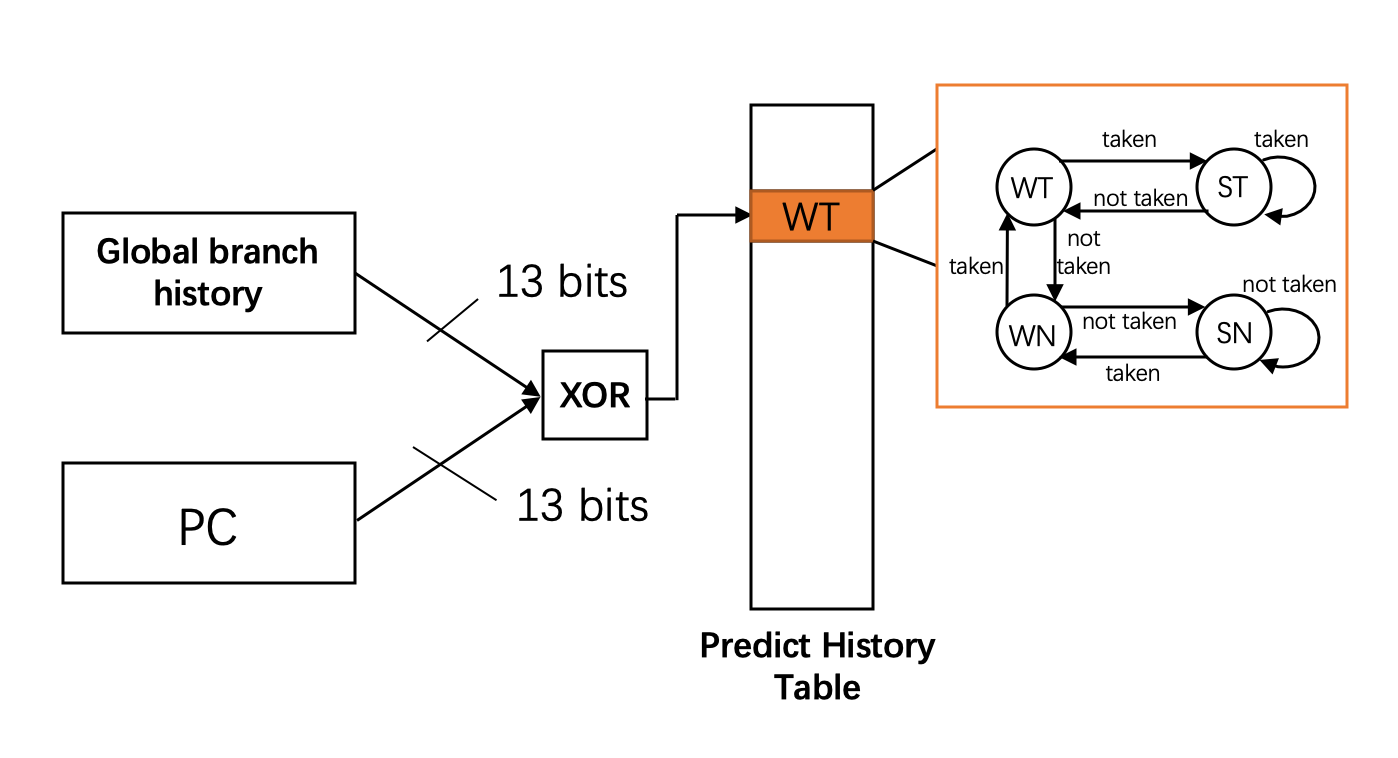
\includegraphics[width=\linewidth]{g-share.png}
\begin{center}
  {\small Figure 1. G-Share predictor}
\end{center}

As Figure 1 indicated, we get the lowest 13-bit PC and global history table and make a XOR calculation. The result is the index for prediction table.
The finite-state machine for prediction result is also contained in Figure 1. G-Share branch predictor employs 2-bit 
history-based branch prediction. The values in prediction table are 2-bit unsigned integers, 
where 0 is strongly not taken(SN), 1 is weakly not taken(WN), 2 is weakly taken(WT), and 3 is strongly taken(ST). We can pick the preduction result from this table.  
\subsection{Tournament branch predictor}
Tournament branch predictor is a hybrid predictor. Why is it called "hybrid"? Because it contains two branch predictor. One is global branch predictor, and the other one is local branch predictor. 
The architecture of Tournament branch predictor is shown in Figure 2. 
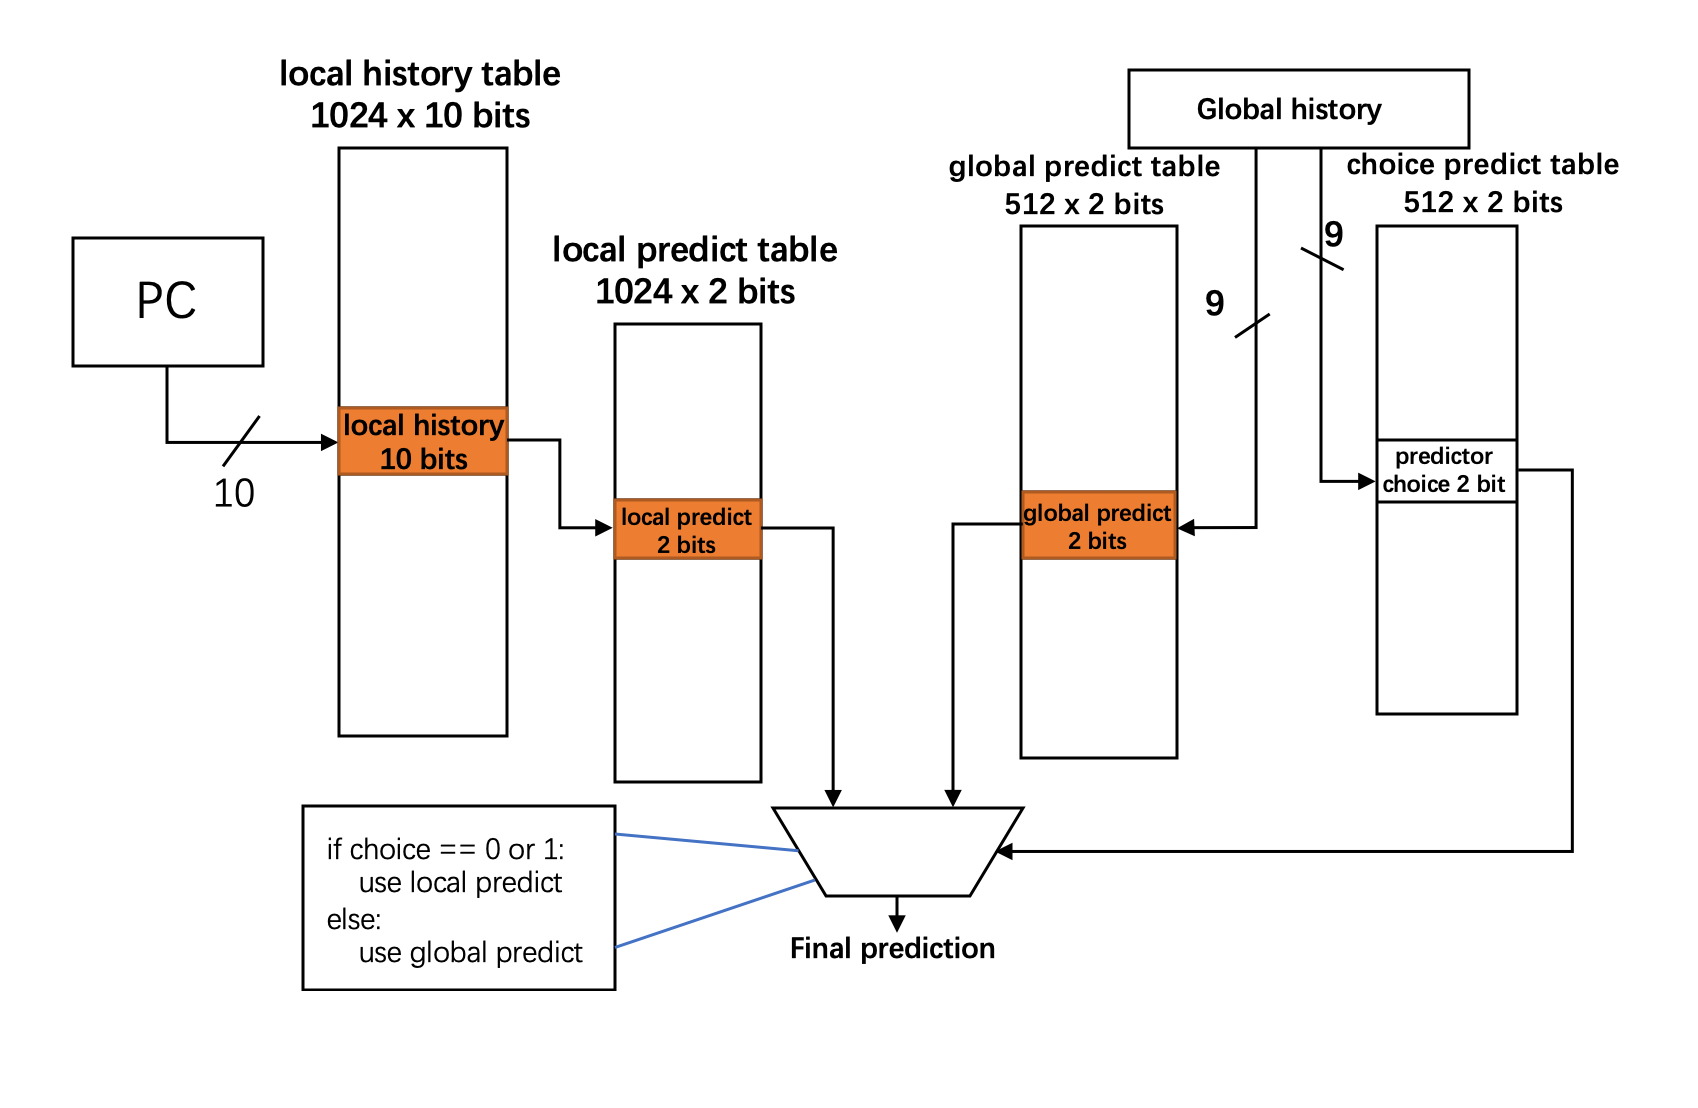
\includegraphics[width=\linewidth]{Tournament.png}
\begin{center}
  {\small Figure 2. Tournament branch predictor}
\end{center}
In this paper, we use Tournament 9:10:10, which means that we assign 9 bits for global history, 10 bits for local history, and 10 bits for PC. We also referred Alpha 21264 Microprocessor Architecture ~\cite{nicepaper5}.  

While making a prediction, the first step is to determine which branch predictor should we use. We firstly pick the lowest 9-bit PC as the index of choice table. Then we pick the value of choice table as our predictor choice. 
The values in choice table employs 2-bit history-based prediction, and it contains four statuses: strongly local, weakly local, weakly global, and strongly global. 

After deciding which branch predictor we use, we then make predictions for branches. If we decide to use local branch predictor, we firstly pick the lowest 10-bit PC address as the index of local history table. 
We get the local history for this PC address. Then we pick the lowest 10-bit local history as the index of local prediction table. The values in local prediction table is the local prediction, which are 2-bit unsigned integers. 
Local prediction has the same set of status as G-Share predictor, containing SN, WN, WT, and ST. 

If we decide to use global predictor, we firstly pick the lowest 9-bit global history as the index of global prediction table. Then we pick the prediction result from global prediction table. 
The values in the global prediction table are 2-bit prediction results, which have the same set of statuses as local predictor. After getting the prediction result, we will have finished prediction with Tournament branch predictor. 
\subsection{Custom Perceptron branch predictor}
Our custom Preceptron branch predictor employs the idea from Dynamic Branch Prediction with Perceptrons paper~\cite{nicepaper4}, which is a micro neural network architecture. The architecture of this branch predictor is shown in Figure 3.
There are two storage structures in this branch predictor. \textbf{The first one is Perceptron Table, which contains weights for different branches. Since we get the lowest 9 bits from PC, there will be 512 entries for Perceptron Table. 
Every group of Perceptron contains 16 weights including a biased variable. Every weight is a 8-bit integer , ranging from -128 to 127. Therefore, the size of Perceptron Table is $512*16*8 = 64k  bits$, which satisfies the project requirement. 
Additionally, the custom Perception contains a global history table, which consists of fifteen 8-bit integers to record the latest 15 outcomes. The size of global history table is $15*8 = 120  bits$, which also 
satisfies the project requirement.}
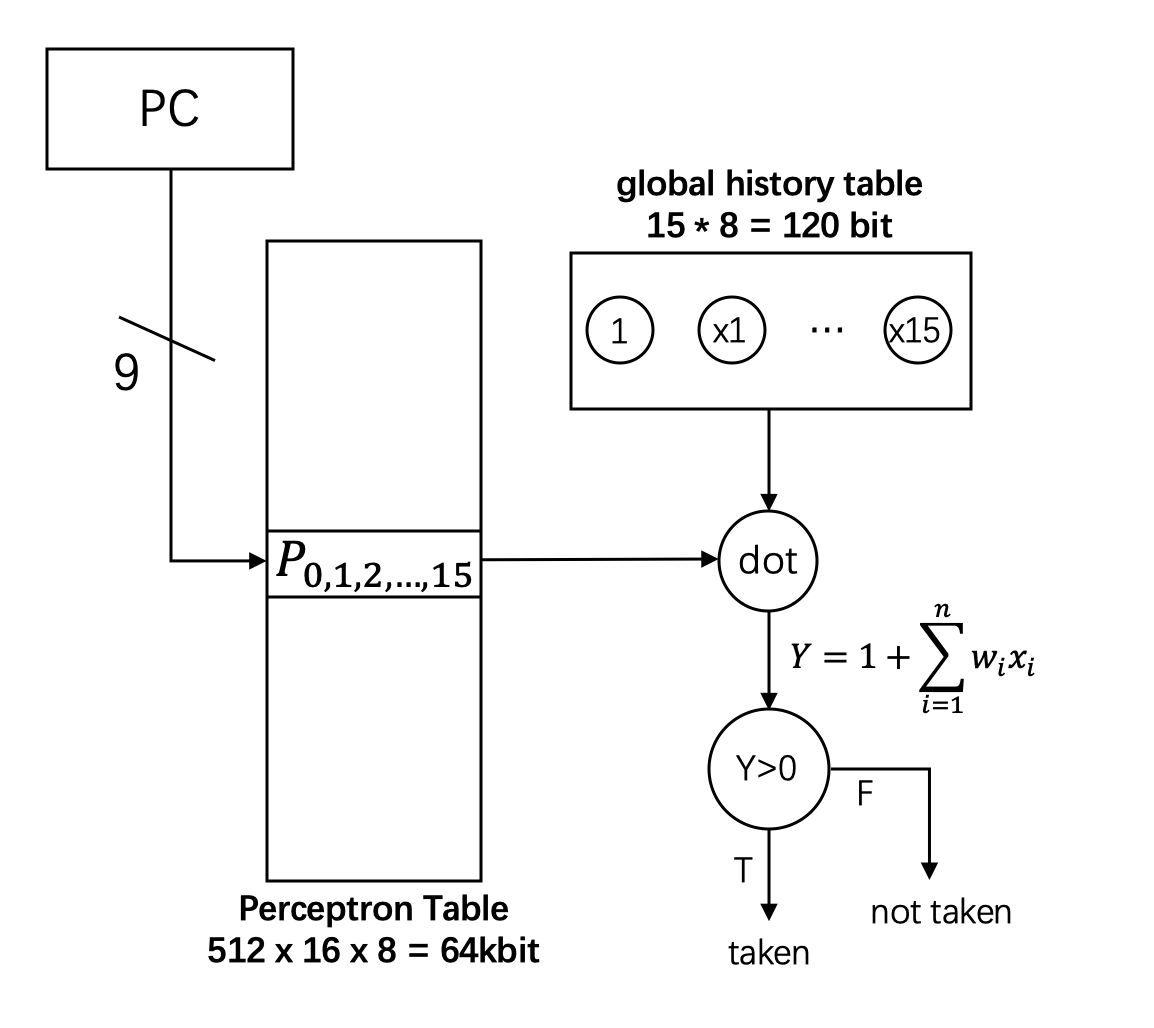
\includegraphics[width=\linewidth]{perceptron.png}
\begin{center}
  {\small Figure 3. Custom Preceptron branch predictor}
\end{center}
For making a prediction, the first step is to get the lowest 9-bit PC as the index of Perceptron Table. Then the predictor will use this index to get the weights from Perceptron Table and make a inner product between Global History Table and the weights.
The inner product result is stored in variable Y. Then the predictor will compare the value of Y with zero. If the value of Y is equal to or greater than zero, then the predictor will predict it as Taken. Otherwise, the predictor will predict it as 
Not Taken. Custom Perceptron branch predictor consumes the fewest data storage, but it performs the best. Really impressive!

\section{implementation}

\section{experiment setup and results}

\section{conclusion}

%%%%%%% -- PAPER CONTENT ENDS -- %%%%%%%%


%%%%%%%%% -- BIB STYLE AND FILE -- %%%%%%%%
\bibliographystyle{IEEEtranS}
\bibliography{refs}
%%%%%%%%%%%%%%%%%%%%%%%%%%%%%%%%%%%%

\end{document}

